\documentclass[11pt]{article}
\usepackage{comment} %includecomment{Antwort} oder excludecomment{Antwort}
\usepackage[ngerman]{babel}\usepackage[babel=true]{microtype}
\usepackage[utf8]{inputenc}
\usepackage[T1]{fontenc}
\usepackage{lmodern}
\usepackage[a4paper,includeheadfoot,
	top=2cm, 
	bottom=2cm, 
	left=2cm, 
	right=2cm]{geometry}
\usepackage{color}
\usepackage{listings}
\usepackage[tikz]{mdframed}%\begin{mybox} \end{mybox}
\usepackage{amsmath,amssymb,amsfonts,amsthm}
\usepackage{graphicx} %\includegraphics[width=0.7\textwidth]{bild.jpg}
\usepackage{placeins} %for \FloatBarrier
\usepackage{caption} 
\usepackage[colorlinks=false,pdfborder={0 0 0}]{hyperref}%Hide RED PDF Border
\usepackage[showonlyrefs]{mathtools}%Math equations erstellen: \numberthis \label{key} abrufen:\ref{key}\eqref{key}
\usepackage{sectsty}
\usepackage{fancyhdr}\pagestyle{fancy}
\usepackage{xcolor} \definecolor{hintergrund}{HTML}{B0C4E3} \definecolor{cobalt}{rgb}{0.0, 0.28, 0.67}


\DeclareMathOperator*{\argmin}{argmin}
\DeclareMathOperator*{\argmax}{argmax}

\newcommand\numberthis{\addtocounter{equation}{1}\tag{\theequation}}
%%%%%%%%%%%%%%%%%%%%%%%%%%%%%%%%%%%%%%%%%%%%%%%%%%%%%%%%%%%%%%%%%%%
%                 Erstellt von Matthias Duch 2017                 %
%                                                                 %
% Programmiersprachen: (ausser den Standardsprachen)              %
% LaTeX, R, Stata                                                 %
%    \%%%%%%%%%%%%%%%%%%%%%%%%%%%%%%%%%%%%%%%%%%%%%%%%%%%%%%%%%%%%%%%%%%%
%                 Erstellt von Matthias Duch 2017                 %
%                                                                 %
% Programmiersprachen: (ausser den Standardsprachen)              %
% LaTeX, R, Stata                                                 %
%    \\input{../1.Vorlesung/Folien/settingsListing}               %
%%%%%%%%%%%%%%%%%%%%%%%%%%%%%%%%%%%%%%%%%%%%%%%%%%%%%%%%%%%%%%%%%%%
\usepackage{listings}
\definecolor{yellow}{RGB}{181,137,0}
\definecolor{red}{RGB}{220,50,47}
\definecolor{violet}{RGB}{108,113,196}
\definecolor{green}{rgb}{0,0.6,0}
\definecolor{gray}{rgb}{0.5,0.5,0.5}

\definecolor{Rblue}{HTML}{0000FF}
\definecolor{myblue}{HTML}{0000FF}




\newcommand{\colcomment}{\color{green}}
\newcommand{\colkeyword}{\color{blue}}
\newcommand{\coltexelem}{\color{green}}
\newcommand{\colnumbers}{\color{gray}}
\newcommand{\colstrings}{\color{violet}}
\newcommand{\colbackgrd}{\color{white}}

\lstset{literate= % Sonderzeichen ersetzen
  {á}{{\'a}}1 {é}{{\'e}}1 {í}{{\'i}}1 {ó}{{\'o}}1 {ú}{{\'u}}1
  {Á}{{\'A}}1 {É}{{\'E}}1 {Í}{{\'I}}1 {Ó}{{\'O}}1 {Ú}{{\'U}}1
  {à}{{\`a}}1 {è}{{\`e}}1 {ì}{{\`i}}1 {ò}{{\`o}}1 {ù}{{\`u}}1
  {À}{{\`A}}1 {È}{{\'E}}1 {Ì}{{\`I}}1 {Ò}{{\`O}}1 {Ù}{{\`U}}1
  {ä}{{\"a}}1 {ë}{{\"e}}1 {ï}{{\"i}}1 {ö}{{\"o}}1 {ü}{{\"u}}1
  {Ä}{{\"A}}1 {Ë}{{\"E}}1 {Ï}{{\"I}}1 {Ö}{{\"O}}1 {Ü}{{\"U}}1
  {â}{{\^a}}1 {ê}{{\^e}}1 {î}{{\^i}}1 {ô}{{\^o}}1 {û}{{\^u}}1
  {Â}{{\^A}}1 {Ê}{{\^E}}1 {Î}{{\^I}}1 {Ô}{{\^O}}1 {Û}{{\^U}}1
  {œ}{{\oe}}1 {Œ}{{\OE}}1 {æ}{{\ae}}1 {Æ}{{\AE}}1 {ß}{{\ss}}1
  {ű}{{\H{u}}}1 {Ű}{{\H{U}}}1 {ő}{{\H{o}}}1 {Ő}{{\H{O}}}1
  {ç}{{\c c}}1 {Ç}{{\c C}}1 {ø}{{\o}}1 {å}{{\r a}}1 {Å}{{\r A}}1
  {€}{{\euro}}1 {£}{{\pounds}}1 {«}{{\guillemotleft}}1
  {»}{{\guillemotright}}1 {ñ}{{\~n}}1 {Ñ}{{\~N}}1 {¿}{{?`}}1
}

\usepackage{accsupp}    
\lstset {
    numberstyle=\tiny\noncopynumber,
}

\newcommand{\noncopynumber}[1]{
    \BeginAccSupp{method=escape,ActualText={}}
    #1
    \EndAccSupp{}
}

% globale Einstellungen
\lstset{ %
  backgroundcolor=\colbackgrd,   % choose the background color; 
  basicstyle=\footnotesize,        % the size of the fonts that are used for the code
  breakatwhitespace=false,         % sets if automatic breaks should only happen at whitespace
  breaklines=true,                 % sets automatic line breaking
  emptylines=1, 
  captionpos=b,                    % sets the caption-position to bottom
  commentstyle=\itshape\colcomment,    % comment style
  deletekeywords={...},            % if you want to delete keywords from the given language
 % escapeinside={\%*}{*)},          % if you want to add LaTeX within your code
  extendedchars=true,              % lets you use non-ASCII characters; for 8-bits encodings only, does not work with UTF-8
  frame=single,	                   % adds a frame around the code
  keepspaces=true,                 % keeps spaces in text, useful for keeping indentation of code (possibly needs columns=flexible)
  keywordstyle=\colkeyword,       % keyword style
  otherkeywords={*,...},           % if you want to add more keywords to the set
  numbers=left,                    % where to put the line-numbers; possible values are (none, left, right)
  numbersep=1pt,                   % how far the line-numbers are from the code
  numberstyle=\sffamily\tiny\color{red!90}\noncopynumber, % the style that is used for the line-numbers
  numberfirstline=true,
  rulecolor=\color{black!70},         % if not set, the frame-color may be changed on line-breaks within not-black text (e.g. comments (green here))
  showspaces=false,                % show spaces everywhere adding particular underscores; it overrides 'showstringspaces'
  showstringspaces=false,          % underline spaces within strings only
  showtabs=false,                  % show tabs within strings adding particular underscores  showtabs=false,                 , % show tabs within strings adding particular underscores
  stepnumber=1,                    % the step between two line-numbers. If it's 1, each line will be numbered
  stringstyle=\colstrings,     % string literal style
  tabsize=2,	                   % sets default tabsize to 2 spaces
  title=\lstname,                   % show the filename of files included with \lstinputlisting; also try caption instead of title
  xleftmargin=3.4pt, % Einschub, durch die Zeilennummerierung bedingt
  xrightmargin=3.4pt,
  %
  alsoletter={.},
  %
  basicstyle=\ttfamily\color{black}, 
  columns=flexible,
}

%%%%%%%%%%%%%%%%%%%%%%%%%%%%%%%%%%%%%%%%%%%%%%%%%%%%%%%%%%%%%%%%%%%
%                           Sprachdefinitionen                    %
%%%%%%%%%%%%%%%%%%%%%%%%%%%%%%%%%%%%%%%%%%%%%%%%%%%%%%%%%%%%%%%%%%%

\lstdefinelanguage{Stata}{
    morekeywords=,
    morekeywords=[2]{cntrade, chinafin, wbopendata, spmap,},
    morekeywords=[3]{regress, summarize, display,},
    morekeywords=[4]{forvalues, if, foreach, set},
    morekeywords=[5]{rnormal, runiform},
    morecomment=[l]{//},
    morecomment=[s]{/*}{*/},
    % The following is used by macros, like `lags'.
    morecomment=[n][keywordstyle]{`}{'},
    morestring=[b]",
    sensitive=true,
}

\lstdefinestyle{Stata}{
  language=Stata,
  keywordstyle=\color{black},
  moredelim=**[is][\color{red}]{@}{@},
}

\lstdefinestyle{R}{%eigentlich nur R, aber aus Kompatibilitat zu alten Versionen
  style=base
}
\newcommand{\CodeSymbol}[1]{\textcolor{red}{#1}}

\lstdefinestyle{base}{
  language=R,
  emptylines=1,
  breaklines=true,
  alsoletter={.},
  basicstyle=\ttfamily\color{black},
  keywordstyle=\color{black},
  moredelim=**[is][\color{red}]{@}{@},
  %otherkeywords={<-,!,!=,~,$,*,\&,+,^,\%,\%/\%,\%*\%,\%\%,<<-,_,/},
%  morekeywords=,
%  morekeywords=[2]{+, chinafin, wbopendata, spmap,},
}

\lstdefinestyle{Latex}{
  language={[LaTeX]TeX},
  %
  moretexcs={geometry, definecolor, textcolor, colorbox, color, pagecolor, fcolorbox, setlength, tableofcontents, subsection, subsubsection, thepage, includegraphics, listoftables, citet, citep, eqref, fnysmbol, nameref, listoffigures, listoftables, url, href, printindex, blindtext, pause, titlepage, frametitle, subtitle, titlepage, usetheme,}, % define Commands
  morekeywords={maketitle}, %Keywords
  %
  texcsstyle=*\coltexelem, % Commandstyle
  moredelim=**[s][\color{yellow}]{[}{]},
}

%Patch issue, that closing parenthesis is not colored, if breaklines=True


               %
%%%%%%%%%%%%%%%%%%%%%%%%%%%%%%%%%%%%%%%%%%%%%%%%%%%%%%%%%%%%%%%%%%%
\usepackage{listings}
\definecolor{yellow}{RGB}{181,137,0}
\definecolor{red}{RGB}{220,50,47}
\definecolor{violet}{RGB}{108,113,196}
\definecolor{green}{rgb}{0,0.6,0}
\definecolor{gray}{rgb}{0.5,0.5,0.5}

\definecolor{Rblue}{HTML}{0000FF}
\definecolor{myblue}{HTML}{0000FF}




\newcommand{\colcomment}{\color{green}}
\newcommand{\colkeyword}{\color{blue}}
\newcommand{\coltexelem}{\color{green}}
\newcommand{\colnumbers}{\color{gray}}
\newcommand{\colstrings}{\color{violet}}
\newcommand{\colbackgrd}{\color{white}}

\lstset{literate= % Sonderzeichen ersetzen
  {á}{{\'a}}1 {é}{{\'e}}1 {í}{{\'i}}1 {ó}{{\'o}}1 {ú}{{\'u}}1
  {Á}{{\'A}}1 {É}{{\'E}}1 {Í}{{\'I}}1 {Ó}{{\'O}}1 {Ú}{{\'U}}1
  {à}{{\`a}}1 {è}{{\`e}}1 {ì}{{\`i}}1 {ò}{{\`o}}1 {ù}{{\`u}}1
  {À}{{\`A}}1 {È}{{\'E}}1 {Ì}{{\`I}}1 {Ò}{{\`O}}1 {Ù}{{\`U}}1
  {ä}{{\"a}}1 {ë}{{\"e}}1 {ï}{{\"i}}1 {ö}{{\"o}}1 {ü}{{\"u}}1
  {Ä}{{\"A}}1 {Ë}{{\"E}}1 {Ï}{{\"I}}1 {Ö}{{\"O}}1 {Ü}{{\"U}}1
  {â}{{\^a}}1 {ê}{{\^e}}1 {î}{{\^i}}1 {ô}{{\^o}}1 {û}{{\^u}}1
  {Â}{{\^A}}1 {Ê}{{\^E}}1 {Î}{{\^I}}1 {Ô}{{\^O}}1 {Û}{{\^U}}1
  {œ}{{\oe}}1 {Œ}{{\OE}}1 {æ}{{\ae}}1 {Æ}{{\AE}}1 {ß}{{\ss}}1
  {ű}{{\H{u}}}1 {Ű}{{\H{U}}}1 {ő}{{\H{o}}}1 {Ő}{{\H{O}}}1
  {ç}{{\c c}}1 {Ç}{{\c C}}1 {ø}{{\o}}1 {å}{{\r a}}1 {Å}{{\r A}}1
  {€}{{\euro}}1 {£}{{\pounds}}1 {«}{{\guillemotleft}}1
  {»}{{\guillemotright}}1 {ñ}{{\~n}}1 {Ñ}{{\~N}}1 {¿}{{?`}}1
}

\usepackage{accsupp}    
\lstset {
    numberstyle=\tiny\noncopynumber,
}

\newcommand{\noncopynumber}[1]{
    \BeginAccSupp{method=escape,ActualText={}}
    #1
    \EndAccSupp{}
}

% globale Einstellungen
\lstset{ %
  backgroundcolor=\colbackgrd,   % choose the background color; 
  basicstyle=\footnotesize,        % the size of the fonts that are used for the code
  breakatwhitespace=false,         % sets if automatic breaks should only happen at whitespace
  breaklines=true,                 % sets automatic line breaking
  emptylines=1, 
  captionpos=b,                    % sets the caption-position to bottom
  commentstyle=\itshape\colcomment,    % comment style
  deletekeywords={...},            % if you want to delete keywords from the given language
 % escapeinside={\%*}{*)},          % if you want to add LaTeX within your code
  extendedchars=true,              % lets you use non-ASCII characters; for 8-bits encodings only, does not work with UTF-8
  frame=single,	                   % adds a frame around the code
  keepspaces=true,                 % keeps spaces in text, useful for keeping indentation of code (possibly needs columns=flexible)
  keywordstyle=\colkeyword,       % keyword style
  otherkeywords={*,...},           % if you want to add more keywords to the set
  numbers=left,                    % where to put the line-numbers; possible values are (none, left, right)
  numbersep=1pt,                   % how far the line-numbers are from the code
  numberstyle=\sffamily\tiny\color{red!90}\noncopynumber, % the style that is used for the line-numbers
  numberfirstline=true,
  rulecolor=\color{black!70},         % if not set, the frame-color may be changed on line-breaks within not-black text (e.g. comments (green here))
  showspaces=false,                % show spaces everywhere adding particular underscores; it overrides 'showstringspaces'
  showstringspaces=false,          % underline spaces within strings only
  showtabs=false,                  % show tabs within strings adding particular underscores  showtabs=false,                 , % show tabs within strings adding particular underscores
  stepnumber=1,                    % the step between two line-numbers. If it's 1, each line will be numbered
  stringstyle=\colstrings,     % string literal style
  tabsize=2,	                   % sets default tabsize to 2 spaces
  title=\lstname,                   % show the filename of files included with \lstinputlisting; also try caption instead of title
  xleftmargin=3.4pt, % Einschub, durch die Zeilennummerierung bedingt
  xrightmargin=3.4pt,
  %
  alsoletter={.},
  %
  basicstyle=\ttfamily\color{black}, 
  columns=flexible,
}

%%%%%%%%%%%%%%%%%%%%%%%%%%%%%%%%%%%%%%%%%%%%%%%%%%%%%%%%%%%%%%%%%%%
%                           Sprachdefinitionen                    %
%%%%%%%%%%%%%%%%%%%%%%%%%%%%%%%%%%%%%%%%%%%%%%%%%%%%%%%%%%%%%%%%%%%

\lstdefinelanguage{Stata}{
    morekeywords=,
    morekeywords=[2]{cntrade, chinafin, wbopendata, spmap,},
    morekeywords=[3]{regress, summarize, display,},
    morekeywords=[4]{forvalues, if, foreach, set},
    morekeywords=[5]{rnormal, runiform},
    morecomment=[l]{//},
    morecomment=[s]{/*}{*/},
    % The following is used by macros, like `lags'.
    morecomment=[n][keywordstyle]{`}{'},
    morestring=[b]",
    sensitive=true,
}

\lstdefinestyle{Stata}{
  language=Stata,
  keywordstyle=\color{black},
  moredelim=**[is][\color{red}]{@}{@},
}

\lstdefinestyle{R}{%eigentlich nur R, aber aus Kompatibilitat zu alten Versionen
  style=base
}
\newcommand{\CodeSymbol}[1]{\textcolor{red}{#1}}

\lstdefinestyle{base}{
  language=R,
  emptylines=1,
  breaklines=true,
  alsoletter={.},
  basicstyle=\ttfamily\color{black},
  keywordstyle=\color{black},
  moredelim=**[is][\color{red}]{@}{@},
  %otherkeywords={<-,!,!=,~,$,*,\&,+,^,\%,\%/\%,\%*\%,\%\%,<<-,_,/},
%  morekeywords=,
%  morekeywords=[2]{+, chinafin, wbopendata, spmap,},
}

\lstdefinestyle{Latex}{
  language={[LaTeX]TeX},
  %
  moretexcs={geometry, definecolor, textcolor, colorbox, color, pagecolor, fcolorbox, setlength, tableofcontents, subsection, subsubsection, thepage, includegraphics, listoftables, citet, citep, eqref, fnysmbol, nameref, listoffigures, listoftables, url, href, printindex, blindtext, pause, titlepage, frametitle, subtitle, titlepage, usetheme,}, % define Commands
  morekeywords={maketitle}, %Keywords
  %
  texcsstyle=*\coltexelem, % Commandstyle
  moredelim=**[s][\color{yellow}]{[}{]},
}

%Patch issue, that closing parenthesis is not colored, if breaklines=True



%Seite Code einbinden:
%\lstinputlisting[language=R,style=base]{Tag1-Uebungsblatt.R}

\addto\captionsngerman{ %Abkürzen der Figureüberschriften
\renewcommand{\figurename}{Abb.}
\renewcommand{\tablename}{Tab.}
}
\lhead{Einführung in \LaTeX}
\chead{SoSe 2017} 
\rhead{Universität Bonn}
\lfoot{} \cfoot{\thepage}% \rfoot{Stand: \today}

\newmdenv[
  outerlinewidth      = 1,
  backgroundcolor     = red!25,
  roundcorner         = 5pt,
  frametitlebelowskip = 0pt,
  skipabove           = 0.5\baselineskip,
  skipbelow           = 0.1\baselineskip,
]{ansbox}

%\renewcommand{\labelenumi}{\alph{enumi})} % nummerieren mit Buchstaben
\newcommand{\code}[1]{\texttt{#1}} % Codeauszeichnung
\newcommand{\qcode}[1]{\glqq \texttt{\textbf{#1}}\grqq}
\newcommand{\bcode}[1]{\texttt{\textbf{#1}}} %fetter Code

\excludecomment{Antwort} %hier stehen lassen! Änderung im eig Dokument

% Überschrift Aufgabenblatt
\usepackage{calc}
\newcommand{\ueberschrift}[1]{\noindent \colorbox{hintergrund}{\parbox[t]{\textwidth - 2 \fboxsep}{\centering \LARGE \textbf{#1:}}}}
\usepackage{titlesec}
\sectionfont{\color{cobalt}} \subsectionfont{\color{cobalt}}
\titleformat{\section}
 {}{}{1em}{{\color{cobalt}\normalfont\bfseries Aufgabe \thesection.}~}
\usepackage{framed}
\newcommand\result[1]{\vspace{\abstandVorResult}\begin{framed}#1\end{framed}}

\usepackage{multirow}
\usepackage{colortbl}		% farbige Tabellen

%zum Ausblenden auskommentieren.
%\renewenvironment{Antwort}{\begin{ansbox}\textbf{Lösung:~}}{\end{ansbox}}
%\aufgabe{Aufgabenstellung}{Beispielcode usw.}{Lösung}
\newcommand{\abstandVorResult}{-15pt}
\newcommand{\abstandVorListing}{-10pt}
\newcommand{\abstandNachListing}{-30pt}

\begin{document}
\ueberschrift{Aufgaben Tag 3}
\section{Erstelle die folgenden Formeln in \LaTeX:}\label{AG:1}
\result{\noindent
\[
f(x)=3x^2-5x+42
\]
\[
x=(x_1,x_2,...,x_n)
\]
\[
r=\frac{a}{b}
\]
\begin{align}
x_i &= a^2 + b^2 & (i<5) \label{eq:1}\\
x_i &= a + b & (i=5) \label{eq:2}
\end{align}
\begin{align}
\pi = 3,1415... \label{eq:1}
\end{align}
}

\begin{Antwort}
\begin{lstlisting}[style=latex]
\[
f(x)=3x^2-5x+42
\]
\[
x=(x_1,x_2,...,x_n)
\]
\[
r=\frac{a}{b}
\]
\begin{align}
x_i &= a^2 + b^2 & (i<5) \label{eq:1}\\
x_i &= a + b & (i=5) \label{eq:2}
\end{align}
\begin{align}
\pi = 3,1415... \label{eq:1}
\end{align}
\end{lstlisting}
\end{Antwort}
\newpage

\section{Versuche, die folgenden Formeln in \LaTeX\, zu übertragen:}
\result{\noindent
Um Seitenlängen in einem rechtwinkligen Dreieck zu bestimmen, werden die Funktionen Sinus ($\sin$) und Kosinus ($\cos$) verwendet. Dabei gilt
\[ \textrm{Sinus eines Winkels} = \frac{\textrm{Gegenkathete des Winkels}}{\textrm{Hypothenuse}} \]
sowie 
\[ \textrm{Kosinus eines Winkels} = \frac{\textrm{Ankathete des Winkels}}{\textrm{Hypothenuse}}. \]
Dies wird auch ausgedrückt durch $\sin(\alpha)=\frac ac$ und $\cos(\alpha)=\frac bc$.\\
Durch die Definition der $e$-Funktion kann man dies auch darstellen als
\begin{align*}
\sin(x) & = \sum_{n=0}^\infty (-1)^n \frac{x^{2n+1}}{(2n+1)!}\\
	& = \frac{x}{1!} - \frac{x^3}{3!} + \frac{x^5}{5!} - \ldots.
\end{align*}
Wir können beobachten, dass gilt
\begin{align}
\sin^{(4n+k)}(0) = 
	\begin{cases}
	0 & \textrm{wenn } k=0 \\
	1 & \textrm{wenn } k=1 \\
	0 & \textrm{wenn } k=2 \\
	-1 & \textrm{wenn } k=3
	\end{cases}	
\end{align}
}

\begin{Antwort}
\begin{lstlisting}[style=latex]
\noindent
Um Seitenlängen in einem rechtwinkligen Dreieck zu bestimmen, werden die Funktionen Sinus ($\sin$) und Kosinus ($\cos$) verwendet. Dabei gilt
\[ \textrm{Sinus eines Winkels} = \frac{\textrm{Gegenkathete des Winkels}}{\textrm{Hypothenuse}} \]
sowie 
\[ \textrm{Kosinus eines Winkels} = \frac{\textrm{Ankathete des Winkels}}{\textrm{Hypothenuse}}. \]
Dies wird auch ausgedrückt durch $\sin(\alpha)=\frac ac$ und $\cos(\alpha)=\frac bc$.\\
Durch die Definition der $e$-Funktion kann man dies auch darstellen als
\begin{align*}
\sin(x) & = \sum_{n=0}^\infty (-1)^n \frac{x^{2n+1}}{(2n+1)!}\\
	& = \frac{x}{1!} - \frac{x^3}{3!} + \frac{x^5}{5!} - \ldots.
\end{align*}
Wir können beobachten, dass gilt
\begin{align}
\sin^{(4n+k)}(0) = 
	\begin{cases}
	0 & \textrm{wenn } k=0 \\
	1 & \textrm{wenn } k=1 \\
	0 & \textrm{wenn } k=2 \\
	-1 & \textrm{wenn } k=3
	\end{cases}	
\end{align}
\end{lstlisting}
\end{Antwort}
\newpage

\section{Erstelle die folgenden Matrizen und die Fallunterscheidung:}
\result{\noindent
Matrizen in Inlineformeln $\begin{pmatrix} 
3 & 2 & 1 \\ 
1 & 0 & 2\\
\end{pmatrix} \cdot 
\begin{pmatrix} 
1 \\ 
0 \\
4
\end{pmatrix}
=
\begin{pmatrix} 
7\\
9
\end{pmatrix}$
sehen sehr schlecht aus. Besser sind diese in abgesetzten Formeln:
\begin{align}
\begin{pmatrix} 
3 & 2 & 1 \\ 
1 & 0 & 2\\
\end{pmatrix} \cdot 
\begin{pmatrix} 
1 \\ 
0 \\
4
\end{pmatrix}
=
\begin{pmatrix} 
7\\
9
\end{pmatrix}
\label{mat:test}
\end{align}
Hier geht der Text nach Matrix \eqref{mat:test} weiter. Das Kronecker-Delta ist wie folgt definiert:
\[
\delta_{ij}:=
\begin{cases}
0& \text{wenn } i \neq j\\
1& \text{wenn } i = j
\end{cases}
\]
Zuletzt verwenden wir eine andere Schreibweise für die Matrix \eqref{mat:test} und lassen die Nummerierung weg.
\begin{align*}
\begin{bmatrix} 
3 & 2 & 1 \\ 
1 & 0 & 2\\
\end{bmatrix} \cdot 
\begin{bmatrix} 
1 \\ 
0 \\
4
\end{bmatrix}
=
\begin{bmatrix} 
7\\
9
\end{bmatrix}
\end{align*}
}

\begin{Antwort}
\begin{lstlisting}[style=latex]
\noindent
Matrizen in Inlineformeln $\begin{pmatrix} 
3 & 2 & 1 \\ 
1 & 0 & 2\\
\end{pmatrix} \cdot 
\begin{pmatrix} 
1 \\ 
0 \\
4
\end{pmatrix}
=
\begin{pmatrix} 
7\\
9
\end{pmatrix}$
sehen sehr schlecht aus. Besser sind diese in abgesetzten Formeln:
\begin{align}
\begin{pmatrix} 
3 & 2 & 1 \\ 
1 & 0 & 2\\
\end{pmatrix} \cdot 
\begin{pmatrix} 
1 \\ 
0 \\
4
\end{pmatrix}
=
\begin{pmatrix} 
7\\
9
\end{pmatrix}
\label{mat:test}
\end{align}
Hier geht der Text nach Matrix \eqref{mat:test} weiter. Das Kronecker-Delta ist wie folgt definiert:
\[
\delta_{ij}:=
\begin{cases}
0& \text{wenn } i \neq j\\
1& \text{wenn } i = j
\end{cases}
\]
Zuletzt verwenden wir eine andere Schreibweise für die Matrix \eqref{mat:test} und lassen die Nummerierung weg.
\begin{align*}
\begin{bmatrix} 
3 & 2 & 1 \\ 
1 & 0 & 2\\
\end{bmatrix} \cdot 
\begin{bmatrix} 
1 \\ 
0 \\
4
\end{bmatrix}
=
\begin{bmatrix} 
7\\
9
\end{bmatrix}
\end{align*}
\end{lstlisting}
\end{Antwort}

\newpage

\section{Arbeiten mit Zitaten:}
\begin{enumerate}
\item Suche auf \url{https://bonnus.ulb.uni-bonn.de/} den Artikel \glqq A theory of reciprocity\grqq~ von Armin Falk
\item Erstelle in ein Dokument, in dem du die genannte Quelle als Bibitem einfügst 
\item Zitiere die Quelle im Text
\end{enumerate}

\begin{minipage}[h]{\textwidth}
Das Ergebnis sollte so ähnlich aussehen:

\fbox{

        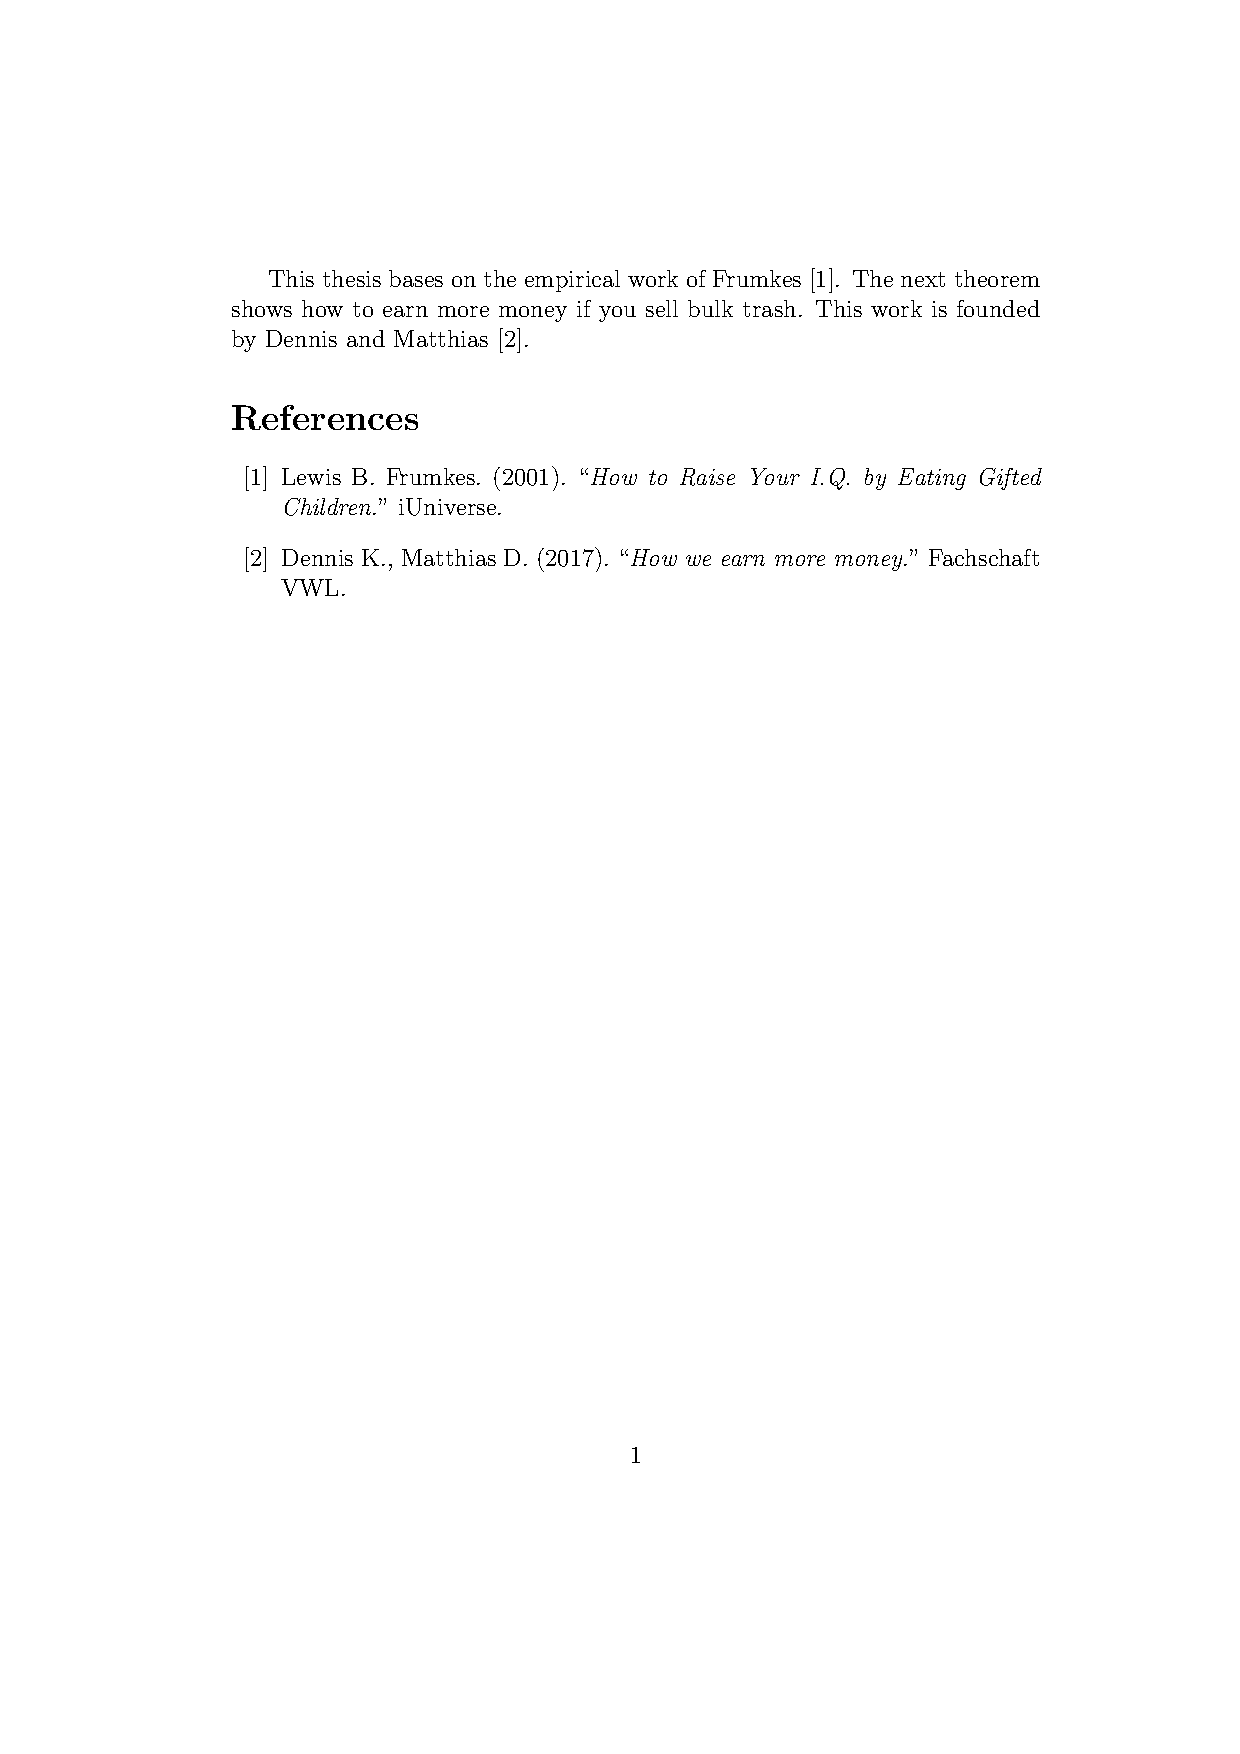
\includegraphics[clip, trim=3cm 19.5cm 0.5cm 4cm, width=1.00\textwidth]{images/Literaturangabe2.pdf}
}
\end{minipage}
\vspace{1cm}

\begin{minipage}[h]{\textwidth}
Verändere die Bibliographie jetzt so, dass in Klammern zuerst der Nachname und dann das Jahr steht:

\fbox{

        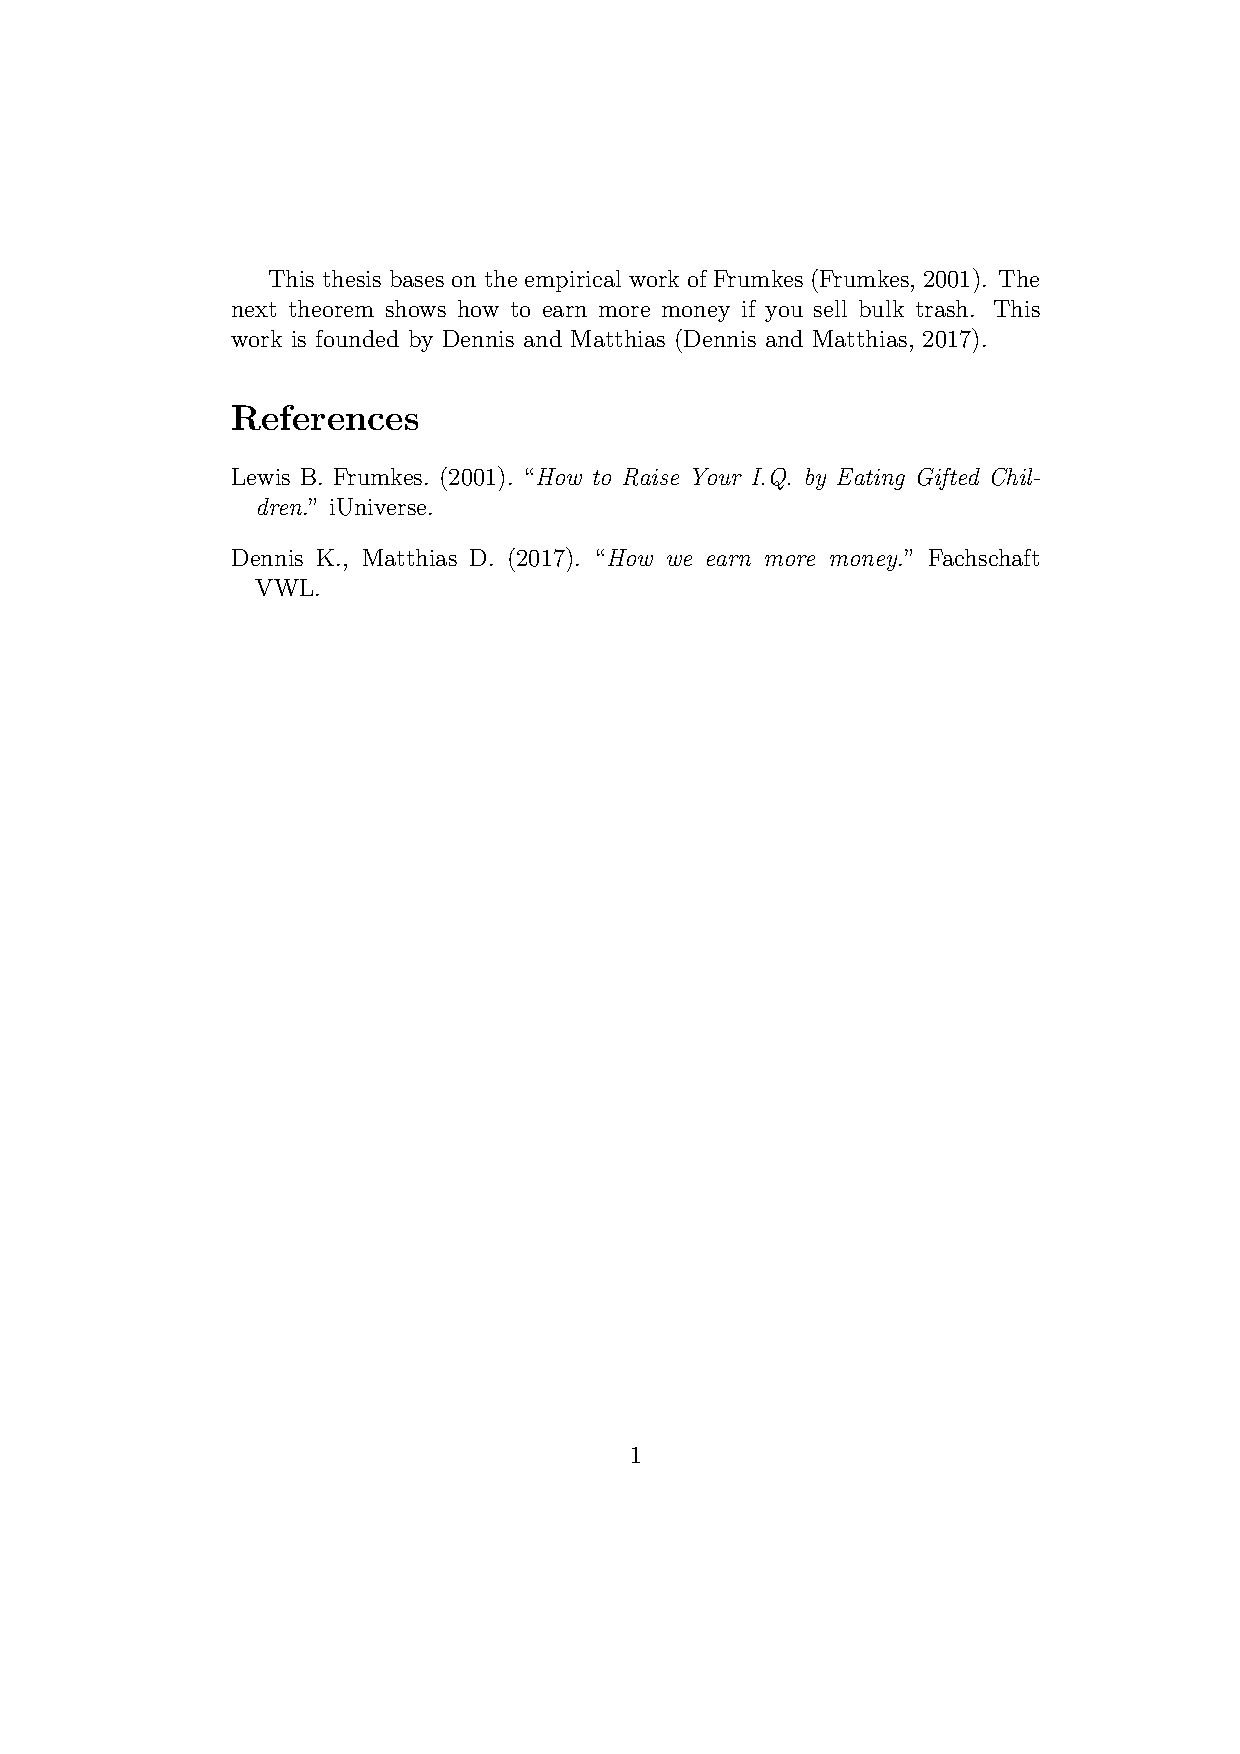
\includegraphics[clip, trim=3cm 19.5cm 0.5cm 4cm, width=1.00\textwidth]{images/Literaturangabe3.pdf}
}
\end{minipage}

\section{Arbeiten mit Fußnoten:}
Platziere die Literaturangaben aus dem letzten Dokument auf einer eigenen Seite und füge eine Fußnote im Text hinzu!

\newpage
\section{Erstelle eine Präsentation, die folgende Kriterien erfüllt:}
\begin{itemize}
  \item die erste Seite soll eine Titelseite sein.
  \item auf der zweiten Seite soll das Inhaltsverzeichnis Punkt für Punkt aufgebaut werden.
  \item auf der dritten Seite soll eine Auflistung von 5 Punkten sein, bei der die Punkte nacheinander erscheinen.
  \item Setze auf die nächsten Folie mehrere Formeln, die nacheinander eingeblenden
  \item Teste verschiedene Themen. Ein Auflistung findest unter \\
  \url{http://deic.uab.es/~iblanes/beamer_gallery/index_by_theme.html}
\end{itemize}

\begin{Antwort}
\begin{lstlisting}[style=latex]
\documentclass[aspectratio = 169]{beamer}
\author{Dennis Kubitza}
\title{Dies ist eine Präsentation}
\usetheme{Singapore}


\begin{document}
\titlepage

\begin{frame}
\tableofcontents
\end{frame}

\section{5 Punkte}
\begin{frame}
Wie man in \eqref{eq:pythagoras} sieht.
	\frametitle{5 Punkte}
	\begin{enumerate}[<+->]
		\item Punkt 1
		\item Punkt 2
		\item Punkt 3
		\item Punkt 4
		\item Punkt 5
	\end{enumerate}
\end{frame}

\section{Formeln}
\begin{frame}
	\frametitle{Formeln}
	\begin{align}
	\label{eq:pythagoras}
	a^2 &= c^2 - b^2 \\
	a^2 + b^2 &= c^2
	\end{align}
	\pause
	\[ \sum_{i=0}^\infty 2^{-i} =2 \]
\end{frame}


\end{document}
\end{lstlisting}
\end{Antwort}

\section{Erstelle eine Referenz zur Gleichung \eqref{eq:2} aus Aufgabe \ref{AG:1}. }
Hinweis: Verwende dazu \lstinline[style=Latex]+\usepackage[colorlinks=false,pdfborder={0 0 0}]{hyperref}+ in der Präambel, \lstinline[style=Latex]+\label{eq:2}+ in der Gleichung um einen Anker zu setzen und rufe diesen schließlich mit \lstinline[style=Latex]+\eqref{eq:2}+ im Text auf! Vergiss nicht, mehrmals auf kompilieren zu klicken, damit die Referenzen so aussehen: ''\texttt{(??)}''!


\section{Zusatzaufgaben}
\textbf{Zusatzaufgabe 1:} Versuche die folgende Formel mit den Nummerierungen und den geschweiften Klammern zu generieren. Erstelle anschließend einen Verweis auf die Gleichung \eqref{gleichung}!\\

Im den komplexen Zahlen gilt:
\begin{align}
e^{\text{i}\varphi} 
	& = \sum_{k=0}^\infty \frac{(\text{i}\varphi)^k}{k!}
	= \sum_{l=0}^\infty \frac{(\text{i}\varphi)^{2l}}{(2l)!}
	  + \sum_{l=0}^\infty \frac{(\text{i}\varphi)^{2l+1}}{(2l+1)!} \\
	& = \underbrace{\sum_{l=0}^\infty (-1)^l \frac{(\text{i}\varphi)^{2l}}{(2l)!}}_{\cos\varphi}
	  + \text{i} \underbrace{\sum_{l=0}^\infty (-1)^l \frac{(\text{i}\varphi)^{2l+1}}{(2l+1)!}}_{\sin\varphi} \label{gleichung}\\
	& = \cos\varphi + \text{i} \sin\varphi
\end{align}

\begin{Antwort}
\begin{lstlisting}[style=latex]
\begin{align}

e^{\text{i}\varphi} 
	& = \sum_{k=0}^\infty \frac{(\text{i}\varphi)^k}{k!}
	= \sum_{l=0}^\infty \frac{(\text{i}\varphi)^{2l}}{(2l)!}
	+ \sum_{l=0}^\infty \frac{(\text{i}\varphi)^{2l+1}}{(2l+1)!} \\
	& = \underbrace{\sum_{l=0}^\infty (-1)^l \frac{(\text{i}\varphi)^{2l}}{(2l)!}}_{\cos\varphi}
	  + \text{i} \underbrace{\sum_{l=0}^\infty (-1)^l \frac{(\text{i}\varphi)^{2l+1}}{(2l+1)!}}_{\sin\varphi} \label{gleichung}\\
	& = \cos\varphi + \text{i} \sin\varphi
\end{align}
\end{lstlisting}
\end{Antwort}
\newpage

\section{Endaufgabe}
Schreibe eine Arbeit (Bachelor/Masterarbeit, Diplomarbeit o.ä.) in \LaTeX. Kehre außerdem den langweiligen, schlechten WYSIWYG-Editoren wie Word o.ä. für immer den Rücken und schreibe fortan alle Texte nur noch in \LaTeX. Du wirst feststellen, dass du mit der Zeit schneller und sicherer in wirst, als du es in einem WYSIWYG-Editor jemals sein könntest.
\end{document}